\documentclass[a4paper]{scrartcl}

\usepackage{float}
\usepackage{tikz}
\usetikzlibrary{arrows,automata}
\usepackage{pgf}
\usepackage[utf8]{inputenc} % this is needed for umlauts
\usepackage[ngerman]{babel} % this is needed for umlauts
\usepackage[T1]{fontenc}    % this is needed for correct output of umlauts in pd
\usepackage{amssymb}
\usepackage{amsmath}
\usepackage{mathrsfs}
\usepackage{dsfont}
\usepackage{graphicx}
\usepackage{fancyhdr}
\usepackage{lastpage}
\usepackage{imakeidx}
\setlength{\parskip}{\medskipamount}
\setlength{\parindent}{0pt}
\usepackage{enumitem}
\usepackage{hyperref}
\usepackage{verbatim}

%%%%%%%%%%%%%%%%%%%%%%%%
% Kopf- und Fusszeilen %
%%%%%%%%%%%%%%%%%%%%%%%%
\pagestyle{fancy}
\lhead{
        Maximilian Roth
}
\chead{Logik-Tutorat Lösungen Blatt 3\\}
\rhead{
        \today{} \\
        Seite \thepage{} von \pageref{LastPage}\\
        
}
\lfoot{}
\cfoot{}
\rfoot{} 

%%%%%%%%%%%%%%%%%%%%%%%%
% Anfang des Dokuments %
%%%%%%%%%%%%%%%%%%%%%%%%

\begin{document}
\section*{Disclaimer}%
\label{sec:disclaimer}
Auch in diesem Dokument können sich Fehler befinden!\\
Sie sind nicht die Musterlösung der Aufgaben, sondern selbst erstellte Lösungen.\\

Als generelle Lektüre kann ich nur das Skript von Markus Junker aus dem WS 17/18 empfehlen:\\
\url{http://home.mathematik.uni-freiburg.de/junker/skripte/InfoLogik.pdf}\\
Hier ist vieles sehr genau und verständlich erklärt.

\section*{}%
\label{sec:aufgabe_1}

    \begin{figure}[H]
        \centering
        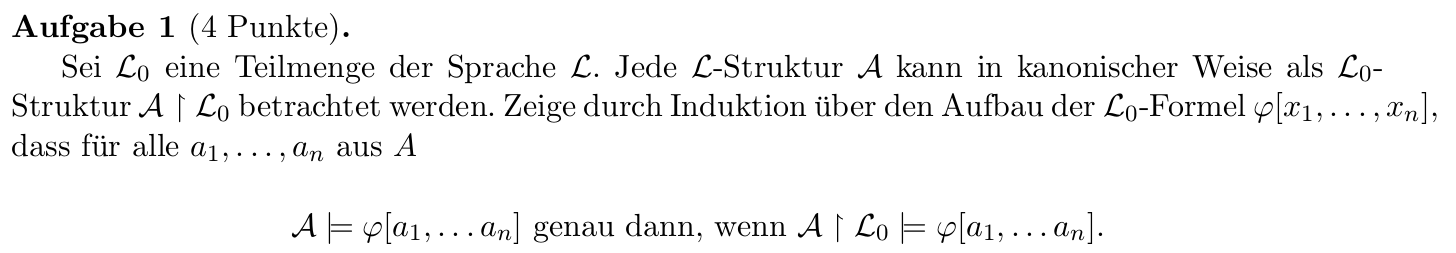
\includegraphics[scale=0.3]{./A-1.png}
        \label{fig:}
    \end{figure}



\section*{}%
\label{sec:aufgabe_2}

    \begin{figure}[H]
        \centering
        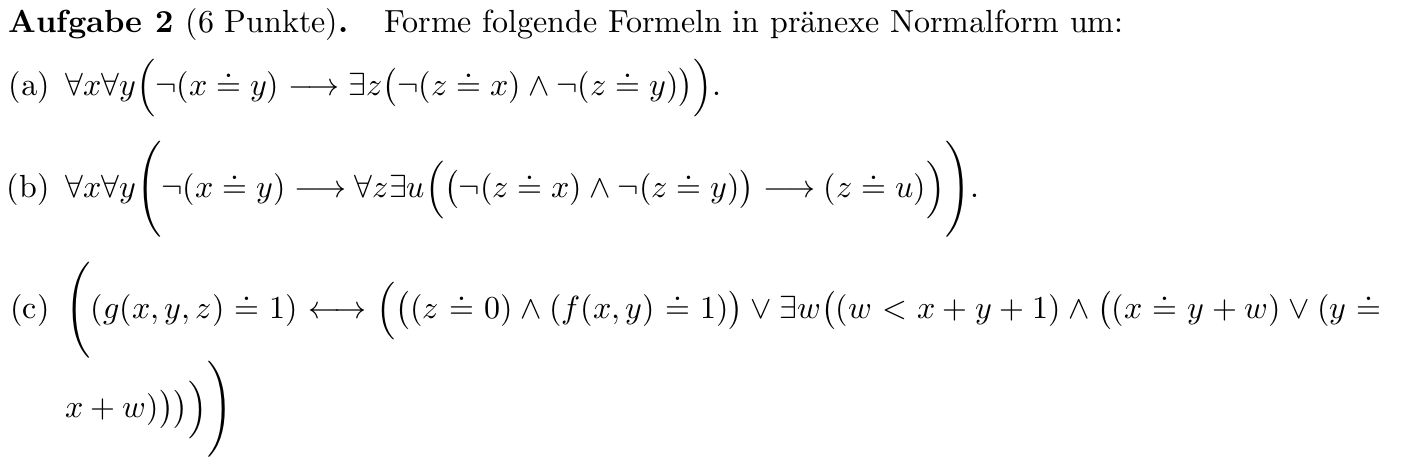
\includegraphics[scale=0.3]{./A-2.png}
        \label{fig:}
    \end{figure}

    \begin{itemize}
        \item a)\\
            $\forall x \forall y (\neg x \doteq y \rightarrow \exists z (\neg z \doteq x \land \neg x \doteq y))$\\
            $\sim \forall x \forall y (x \doteq y \lor \exists z (\neg z \doteq x \land \neg x \doteq y))$\\
            $\sim \forall x \forall y \exists z (x \doteq y \lor (\neg z \doteq x \land \neg x \doteq y))$\\

        \item b)\\
            $\forall x \forall y (\neg x \doteq y \rightarrow \forall z \exists u ((\neg z \doteq x \land \neg z \doteq y) \rightarrow z \doteq u))$\\
            $\sim \forall x \forall y (x \doteq y \lor \forall z \exists u ((\neg z \doteq x \land \neg z \doteq y) \rightarrow z \doteq u))$\\
            $\sim \forall x \forall y \forall z \exists u (x \doteq y \lor ((\neg z \doteq x \land \neg z \doteq y) \rightarrow z \doteq u))$\\

        \item c)\\
            $(gxyz \doteq 1 \leftrightarrow ((z \doteq 0 \land fxy \doteq 1) \lor \exists w (w < x + y + 1 \land (x \doteq y + w \lor y \doteq x + w))))$\\
            \\$\sim ((gxyz \doteq 1 \rightarrow ((z \doteq 0 \land fxy \doteq 1) \lor \exists w (w < x + y + 1 \land (x \doteq y + w \lor y \doteq x + w))))
            \land (((z \doteq 0 \land fxy \doteq 1) \lor \exists w (w < x + y + 1 \land (x \doteq y + w \lor y \doteq x + w))) \rightarrow gxyz \doteq 1))$\\
            \\$\sim ((\neg gxyz \doteq 1 \lor ((z \doteq 0 \land fxy \doteq 1) \lor \exists w (w < x + y + 1 \land (x \doteq y + w \lor y \doteq x + w))))
            \land (\neg((z \doteq 0 \land fxy \doteq 1) \lor \exists w (w < x + y + 1 \land (x \doteq y + w \lor y \doteq x + w))) \lor gxyz \doteq 1))$\\
            \\$\sim \exists w ((\neg gxyz \doteq 1 \lor ((z \doteq 0 \land fxy \doteq 1) \lor (w < x + y + 1 \land (x \doteq y + w \lor y \doteq x + w))))
            \land (\neg((z \doteq 0 \land fxy \doteq 1) \lor \exists w (w < x + y + 1 \land (x \doteq y + w \lor y \doteq x + w))) \lor gxyz \doteq 1))$\\
            \\$\sim \exists w ((\neg gxyz \doteq 1 \lor ((z \doteq 0 \land fxy \doteq 1) \lor (w < x + y + 1 \land (x \doteq y + w \lor y \doteq x + w))))
            \land (\neg \exists w((z \doteq 0 \land fxy \doteq 1) \lor (w < x + y + 1 \land (x \doteq y + w \lor y \doteq x + w))) \lor gxyz \doteq 1))$\\
            \\$\sim \exists w ((\neg gxyz \doteq 1 \lor ((z \doteq 0 \land fxy \doteq 1) \lor (w < x + y + 1 \land (x \doteq y + w \lor y \doteq x + w))))
            \land (\forall w \neg ((z \doteq 0 \land fxy \doteq 1) \lor (w < x + y + 1 \land (x \doteq y + w \lor y \doteq x + w))) \lor gxyz \doteq 1))$\\
            \\$\sim \exists w \forall v((\neg gxyz \doteq 1 \lor ((z \doteq 0 \land fxy \doteq 1) \lor (w < x + y + 1 \land (x \doteq y + w \lor y \doteq x + w))))
            \land (\neg ((z \doteq 0 \land fxy \doteq 1) \lor (v < x + y + 1 \land (x \doteq y + v \lor y \doteq x + v))) \lor gxyz \doteq 1))$\\


    \end{itemize}


\section*{}%
\label{sec:aufgabe_3}

    \begin{figure}[H]
        \centering
        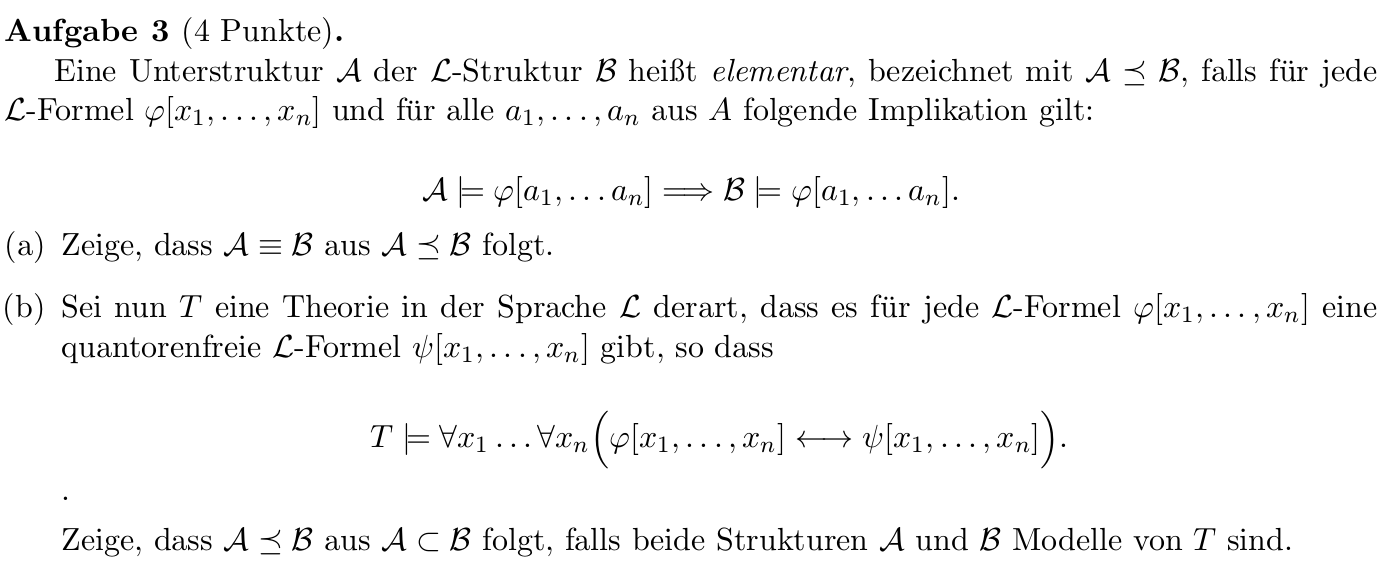
\includegraphics[scale=0.3]{./A-3.png}
        \label{fig:}
    \end{figure}

\section*{}%
\label{sec:aufgabe_4}

    \begin{figure}[H]
        \centering
        
\includegraphics[scale=0.3]{./A-4-1.png}
        \label{fig:}
    \end{figure}

    \begin{figure}[H]
        \centering
        
\includegraphics[scale=0.3]{./A-4-2.png}
        \label{fig:}
    \end{figure}

\end{document}
